\subsection{M.PC.PV - Planned Value e M.PC.EV - Earned Value}

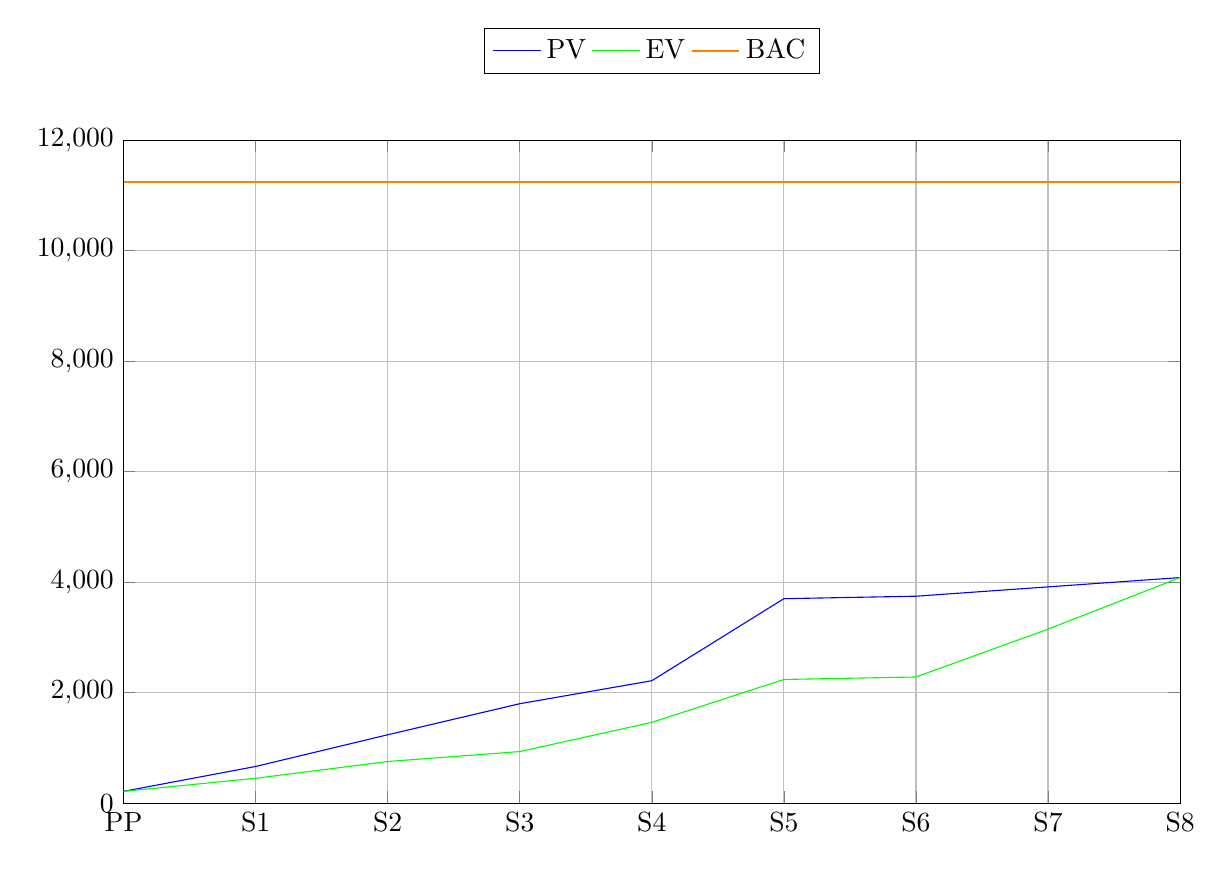
\begin{tikzpicture}
    \begin{axis}[
        width=15cm, height=10cm,
        ymin=0, ymax=12000,
        xmin=0, xmax=8,
        xtick={0, 1, 2, 3, 4, 5, 6, 7, 8},
        xticklabels={ PP, S1, S2, S3, S4, S5, S6, S7, S8},
        xlabel={},
        ylabel={},
        grid=major,
        scaled ticks=false,
        legend style={at={(0.5,1.1)}, anchor=south, legend columns=-1},
    ]
    \addplot[color=blue] coordinates {(0, 213.75) (1, 663.75) (2, 1237.5) (3, 1800) (4, 2216.25) (5, 3701.25) (6, 3746.25) (7, 3915) (8, 4083.75) };
    \addlegendentry{PV}
    \addplot[color=green] coordinates {(0, 213.75) (1, 450) (2, 753.75) (3, 933.75) (4, 1462.5) (5, 2238.75) (6, 2283.75) (7, 3150) (8, 4083.75) };
    \addlegendentry{EV}
    \addplot[orange, thick] coordinates {(0, 11250) (8, 11250)};
    \addlegendentry{BAC}
    \end{axis}
\end{tikzpicture}
\subsubsection{RTB}
Come visibile dal grafico l'\glossario{Earned Value} è sempre inferiore rispetto al \glossario{Planned Value}, indicando una pianificazione 
mal riuscita da parte del gruppo.